% -*- latex -*-
%%%%%%%%%%%%%%%%%%%%%%%%%%%%%%%%%%%%%%%%%%%%%%%%%%%%%%%%%%%%%%%%
%%%%%%%%%%%%%%%%%%%%%%%%%%%%%%%%%%%%%%%%%%%%%%%%%%%%%%%%%%%%%%%%
%%%%
%%%% This text file is part of the source of 
%%%% `Parallel Programming in MPI and OpenMP'
%%%% by Victor Eijkhout, copyright 2012-6
%%%%
%%%% mpi.tex : leftover MPI topics
%%%%
%%%%%%%%%%%%%%%%%%%%%%%%%%%%%%%%%%%%%%%%%%%%%%%%%%%%%%%%%%%%%%%%
%%%%%%%%%%%%%%%%%%%%%%%%%%%%%%%%%%%%%%%%%%%%%%%%%%%%%%%%%%%%%%%%

\Level 0 {Synchronization}
\index{synchronization!in MPI|(}

MPI programs conform to the \ac{SPMD} model, and this means that events
in one process can be unrelated in time to events in another process.
Any \emph{synchronization} that happens is induced by communication 
and other MPI mechanisms. By synchronization here we mean any sort of
temporal ordering of events in different processes.

You have already seen some mechanisms.
\begin{enumerate}
\item In blocking communication, the receive call does not return until the send call has completed.
\item In non-blocking communication, the wait on a receive request will not return 
  until the send has been completed.
\item In one-sided communication, the fence mechanism impose a certain ordering on events.
\end{enumerate}

Another synchronization mechanism is induced by the \emph{barrier}\index{barrier!in MPI}
mechanism. However, while an \indexmpishow{MPI_Barrier} call guarantees that all processes have
reached a certain location in their source, this does not necessarily imply anything about 
message traffic. Consider this example
\begin{quotation}
  \begin{tabular}{|l|l|l|}
    \hline
    Proc 0 & Proc 1 & Proc 2\\
    \hline
    Isend to 1 & Irecv from any source & \\
    Barrier    & Barrier               & Barrier \\
    Wait for send request & wait for recv request & Isend to 1 \\
                          & (another wildcard recv) & wait for send request \\
    \hline
  \end{tabular}
\end{quotation}
The unexpected behaviour here is that the (first) receive on process~1
can be matched with the send on process~2: the barrier on process~1 only guarantees that the 
receive instruction was performed, not the actual transfer. For that you need the \n{MPI_Wait}
call, which is after the barrier.

\index{synchronization!in MPI|)}

\Level 0 {Error handling}
\label{sec:mpi:error}

Errors in normal programs can be tricky to deal with; errors in
parallel programs can be even harder. This is because in addition to
everything that can go wrong with a single executable (floating point
errors, memory violation) you now get errors that come from faulty
interaction between multiple executables.

A few examples of what can go wrong:
\begin{itemize}
\item MPI errors: an MPI routine can abort for various reasons, such
  as receiving much more data than its buffer can accomodate. Such
  errors, as well as the more common type mentioned above, typically
  cause your whole execution to abort. That is, if one incarnation of
  your executable aborts, the MPI runtime will kill all others.
\item Deadlocks and other hanging executions: there are various
  scenarios where your processes individually do not abort, but are all
  waiting for each other. This can happen if two processes are both
  waiting for a message from each other, and this can be helped by
  using non-blocking calls. In another scenario, through an error in
  program logic, one process will be waiting for more messages
  (including non-blocking ones) than are sent to it.
\end{itemize}

The MPI library has a general mechanism for dealing with errors that
it detects. The default behaviour, where the full run is aborted, is
equivalent to your code having the following
call\indexmpi{MPI_Comm_set_errhandler}\footnote{The routine
  \n{MPI\_Errhandler\_set} is deprecated.}:
\begin{verbatim}
MPI_Comm_set_errhandler(MPI_COMM_WORLD,MPI_ERRORS_ARE_FATAL);
\end{verbatim}
Another simple possibility is to specify
\begin{verbatim}
MPI_Comm_set_errhandler(MPI_COMM_WORLD,MPI_ERRORS_RETURN);
\end{verbatim}
which gives you the opportunity to write code that handles the error
return value. The values \indexmpidef{MPI_ERRORS_ARE_FATAL} and
\indexmpidef{MPI_ERRORS_RETURN} are of type \indexmpidef{MPI_Errhandler}.

In most cases where an MPI error occurs a complete abort is the
sensible thing, since there are few ways to recover. The second
possibility can for instance be used to print out debugging
information:
\begin{verbatim}
int ierr;
ierr = MPI_Something();
if (ierr!=0) {
    // print out information about what your programming is doing
    MPI_Abort();
}
\end{verbatim}
For instance,
\begin{verbatim}
Fatal error in MPI_Waitall: 
See the MPI_ERROR field in MPI_Status for the error code
\end{verbatim}
You could then retrieve the \indexmpishow{MPI_ERROR} field of the
status, and print out an error string with \indexmpidef{MPI_Error_string}:
\begin{verbatim}
MPI_Comm_set_errhandler(MPI_COMM_WORLD,MPI_ERRORS_RETURN);
ierr = MPI_Waitall(2*ntids-2,requests,status);
if (ierr!=0) {
   char errtxt[200];
   for (int i=0; i<2*ntids-2; i++) {
       int err = status[i].MPI_ERROR; int len=200;
       MPI_Error_string(err,errtxt,&len);
       printf("Waitall error: %d %s\n",err,errtxt);
   }
   MPI_Abort(MPI_COMM_WORLD,0);
}
\end{verbatim}
One cases where errors can be handled is that of \emph{MPI file
  I/O}\indexterm{MPI!I/O}: if an output file has the wrong
permissions, code can possibly progress without writing data, or
writing to a temporary file.

MPI operators (\indexmpishow{MPI_Op}) do not return an error code. In case of
an error they call \n{MPI_Abort}; if \indexmpishow{MPI_ERRORS_RETURN}
is the error handler, errors may be silently ignore.

You can create your own error handler with
\indexmpidef{MPI_Comm_create_errhandler}, which is then installed with
\indexmpishow{MPI_Comm_set_errhandler}. You can retrieve the error
handler with \indexmpishow{MPI_Comm_get_errhandler}.

\Level 0 {Fortran issues}
\label{sec:mpi-fortran}
\index{MPI!Fortran issues|see{Fortran, MPI issues}}
\index{Fortran!MPI issues|(}

MPI is typically written in C, what if you program \emph{Fortran}?

\Level 1 {Kind-defined types}
\label{sec:f90-kind}

If your Fortran code uses \n{KIND} to define scalar types with
specified precision, these do not in general correspond to any
predefined MPI datatypes. Hence the following routines exist to make
\emph{MPI equivalences of Fortran scalar types}%
\index{Fortran!MPI equivalences of scalar types}:

\mpiRoutineRef{MPI_Type_create_f90_integer}
\mpiRoutineRef{MPI_Type_create_f90_real}
\mpiRoutineRef{MPI_Type_create_f90_complex}

Examples:
\begin{verbatim}
INTEGER ( KIND = SELECTED_INTEGER_KIND(15) ) , &
 DIMENSION(100) :: array INTEGER :: root , integertype , error 

CALL MPI_Type_create_f90_integer( 15 , integertype , error )
CALL MPI_Bcast ( array , 100 ,
 & integertype , root ,
 & MPI_COMM_WORLD , error )

REAL ( KIND = SELECTED_REAL_KIND(15 ,300) ) , &
 DIMENSION(100) :: array
CALL MPI_Type_create_f90_real( 15 , 300 , realtype , error )

COMPLEX ( KIND = SELECTED_REAL_KIND(15 ,300) ) , &
 DIMENSION(100) :: array 
CALL MPI_Type_create_f90_complex( 15 , 300 , complextype , error )
\end{verbatim}

\Level 1 {Assumed-shape arrays}\index{Fortran!assumed-shape arrays in MPI}

Use of other than contiguous data, for instance \n{A(1:N:2)}, was a
problem in MPI calls, especially non-blocking ones. In that case it
was best to copy the data to a contiguous array. This has been fixed
in MPI3.

\begin{itemize}
\item Fortran routines have the same prototype as C~routines except for the addition
  of an integer error parameter.
\item The call for \indexmpishowsub{MPI_Init}{in Fortran} does not have the commandline arguments;
  they need to be handled separately.
\item The routine \indexmpishow{MPI_Sizeof} is only available in Fortran, it provides the 
  functionality of the C/C++ operator \indextermtt{sizeof}.
\end{itemize}

\index{Fortran!MPI issues|)}

\Level 0 {Fault tolerance}
\label{mpi:tolerant}

Processors are not completely reliable, so it may happen that one
`breaks': for software or hardware reasons it becomes
unresponsive. For an MPI program this means that it becomes impossible
to send data to it, and any collective operation involving it will
hang. Can we deal with this case? Yes, but it involves some
programming.

First of all, one of the possible MPI error return codes
(section~\ref{mpi:error}) is \n{MPI_ERR_COMM}, which can be returned
if a processor in the communicator is unavailable. You may want to
catch this error, and add a `replacement processor' to the
program. For this, the \indexmpishow{MPI_Comm_spawn} can be used
(see~\ref{sec:mpi-dynamic} for details).
%
But this requires a change of program design: the communicator
containing the new process(es) is not part of the
old \n{MPI_COMM_WORLD}, so it is better to set up your code as a
collection of inter-communicators to begin with.

\Level 0 {Context information}
\label{sec:context}

The \indextermbus{MPI}{version} is available through two parameters
\indexmpishow{MPI_VERSION} and \indexmpishow{MPI_SUBVERSION}
or the function \indexmpishow{MPI_Get_version}.

\Level 0 {Timing}
\label{sec:mpi-timing}
\index{timing!MPI|(}

Timing of parallel programs is tricky. On each node you can use a timer,
typically based on some \ac{OS} call. MPI supplies its own routine
\indexmpishow{MPI_Wtime} which gives \indexterm{wall clock time}.
Normally you don't worry about the starting point for this timer: 
you call it before and after an event and subtract the values.
\begin{verbatim}
t = MPI_Wtime();
// something happens here
t = MPI_Wtime()-t;
\end{verbatim}
If you execute this on a single processor you get fairly reliable
timings, except that you would need to subtract the overhead for the
timer. This is the usual way to measure timer overhead:
\begin{verbatim}
t = MPI_Wtime();
// absolutely nothing here
t = MPI_Wtime()-t;
\end{verbatim}

\Level 1 {Global timing}

However, if you try to time a parallel application you will most likely
get different times for each process, so you would have to take the
average or maximum.  Another solution is to synchronize the processors
by using a \indexterm{barrier}\indexmpi{MPI_Barrier}:
\begin{verbatim}
MPI_Barrier(comm)
t = MPI_Wtime();
// something happens here
MPI_Barrier(comm)
t = MPI_Wtime()-t;
\end{verbatim}

\begin{exercise}
  This scheme also has some overhead associated with it. How would you measure that?
\end{exercise}

\Level 1 {Local timing}
\label{sec:ping-time}

Now suppose you want to measure the time for a single send. It is not possible
to start a clock on the sender and do the second measurement on the receiver,
because the two clocks need not be synchronized. Usually a \indexterm{ping-pong} is 
done: 
\begin{verbatim}
if ( proc_source ) {
  MPI_Send( /* to target */ );
  MPI_Recv( /* from target */ );
else if ( proc_target ) {
  MPI_Recv( /* from source */ );
  MPI_Send( /* to source */ );
}
\end{verbatim}

\begin{exercise}
  Why is it generally not a good idea to use processes 0 and~1 for the
  source and target processor?  Can you come up with a better guess?
\end{exercise}

No matter what sort of timing you are doing, it is good to know the accuracy of your timer.
The routine \indexmpishow{MPI_Wtick} gives the smallest possible timer increment.
If you find that your timing result is too close to this `tick', you need to find a better timer
(for CPU measurements there are cycle-accurate timers), or you need to increase
your running time, for instance by increasing the amount of data.

\index{timing!MPI|)}

\Level 0 {Profiling}
\label{sec:profile}

MPI allows you to write your own profiling interface. To make this possible,
every routine \n{MPI_Something} calls a routine \n{PMPI_Something} that 
does the actual work. You can now write your \n{MPI_...} routine
which calls \indexmpishow{PMPI_...}, and inserting your own profiling calls.
\begin{figure}
  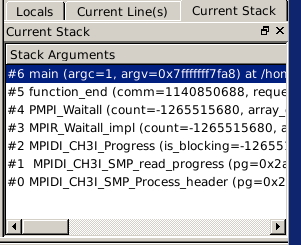
\includegraphics[scale=.7]{graphics/pmpi}
  \caption{A stack trace, showing the \texttt{PMPI} calls.}
  \label{fig:pmpi}
\end{figure}
As you can see in figure~\ref{fig:pmpi}, normally only the \n{PMPI} routines
show up in the stack trace.

Does the standard mandate this?

\Level 0 {Determinism}
\label{sec:mpi-semantics}
\index{MPI!semantics|(}

MPI processes are only synchronized to a certain extent, so you may
wonder what guarantees there are that running a code twice will give
the same result.  You need to consider two cases: first of all, if the
two runs are on different numbers of processors there are already
numerical problems; see~\HPSCref{sec:roundoff-parallel}.

Let us then limit ourselves to two runs on the same set of processors. 
In that case, MPI is deterministic as long as you do not use 
wildcards such as \indexmpishow{MPI_ANY_SOURCE}. Formally, 
MPI messages are `non-overtaking': two messages between the same
sender-receiver pair will arrive in sequence.
Actually, they may not arrive in sequence: they are \emph{matched}\index{matching}
in sequence in the user program. If the second message is much smaller than the first,
it may actually arrive earlier in the lower transport layer.

\index{MPI!semantics|)}

\Level 0 {Progress}
\index{progress|(}

Non-blocking communication implies that messages make \emph{progress}
while computation is going on. However, communication of this sort can 
typically not be off-loaded to the network card, so it has to be done by 
a process. This requires a separate thread of execution, with
obvious performance problems. Therefore, in practice overlap may
not actually happen, and for the message to make progress
it is necessary for the MPI library to become active occasionally.
For instance, people have inserted dummy \n{MPI_Probe} calls.

A similar problem arises with passive target synchronization:
it is possible that the origin process may hang until 
the target process makes an MPI call.

\index{progress|)}

\Level 0 {Subtleties with processor synchronization}
\label{sec:handshake}

Blocking communication involves a complicated dialog between the two
processors involved. Processor one says `I~have this much data to
send; do you have space for that?', to which processor two replies
`yes, I~do; go ahead and send', upon which processor one does the
actual send. This back-and-forth (technically known as
a \indexterm{handshake}) takes a certain amount of communication
overhead. For this reason, network hardware will sometimes forgo the
handshake for small messages, and just send them regardless, knowing
that the other process has a small buffer for such occasions.

%This behaviour is not dictated by the standard: it is up to the implementation
%to make this optimization for small messages.

One strange side-effect of this strategy is that a code that
should \indexterm{deadlock} according to the MPI specification does
not do so. In effect, you may be shielded from you own programming
mistake! Of course, if you then run a larger problem, and the small
message becomes larger than the threshold, the deadlock will suddenly
occur. So you find yourself in the situation that a bug only manifests
itself on large problems, which are usually harder to debug. In this
case, replacing every \n{MPI_Send} with a \indexmpishow{MPI_Ssend} will force the
handshake, even for small messages.

Conversely, you may sometimes wish to avoid the handshake on large
messages. MPI as a solution for this: the \indexmpishow{MPI_Rsend} (`ready
send') routine sends its data immediately, but it needs the receiver
to be ready for this. How can you guarantee that the receiving process
is ready? You could for instance do the following (this uses
non-blocking routines, which are explained below in
section~\ref{sec:nonblocking}):
\begin{verbatim}
if ( receiving ) {
  MPI_Irecv()   // post non-blocking receive
  MPI_Barrier() // synchronize
else if ( sending ) {
  MPI_Barrier() // synchronize
  MPI_Rsend()   // send data fast
\end{verbatim}
When the barrier is reached, the receive has been posted, so it is safe 
to do a ready send. However, global barriers are not a good idea.
Instead you would just synchronize the two processes involved.
\begin{exercise}
  Give pseudo-code for a scheme where you synchronize the two
  processes through the exchange of a blocking zero-size message.
\end{exercise}

\Level 0 {The origin of one-sided communication in ShMem}

The \indextermbus{Cray}{T3E} had a library called \indexterm{shmem}
which offered a type of shared memory. Rather than having a true
global address space it worked by supporting variables that were
guaranteed to be identical between processors, and indeed, were
guaranteed to occupy the same location in memory. Variables could be
declared to be shared a `symmetric' pragma or directive; their values
could be retrieved or set by \n{shmem_get} and \n{shmem_put} calls.

\Level 0 {Literature}

Online resources:
\begin{itemize}
\item MPI 1 Complete reference:\\ \url{http://www.netlib.org/utk/papers/mpi-book/mpi-book.html}
\item Official MPI documents:\\ \url{http://www.mpi-forum.org/docs/}
\item List of all MPI routines:\\ \url{http://www.mcs.anl.gov/research/projects/mpi/www/www3/}
\end{itemize}

Tutorial books on MPI:
\begin{itemize}
\item Using MPI~\cite{Gropp:UsingMPI1} by some of the original authors.
\end{itemize}

\endinput

Examples: 
compute pi
mandelbrot set
